\section{Appendix}

\subsection{Code}

\subsection{Figures}

\begin{figure}[h]
\centering
\begin{subfigure}{.5\textwidth}
  \centering
  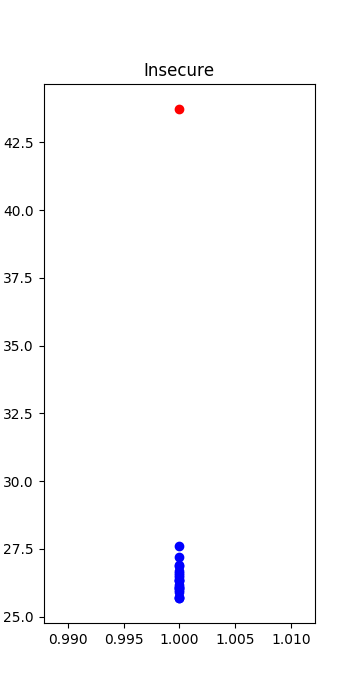
\includegraphics[width=.7\linewidth]{figures/insecure0.png}
  \caption{Na\"ive implementation}
  \label{fig:sub1}
\end{subfigure}%
\begin{subfigure}{.5\textwidth}
  \centering
  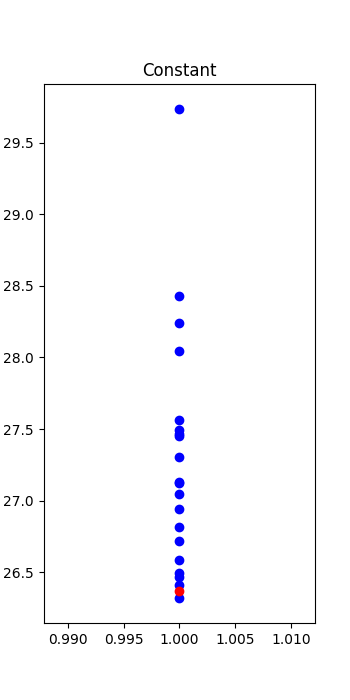
\includegraphics[width=.7\linewidth]{figures/constant0.png}
  \caption{Constant Time implementation}
  \label{fig:sub2}
\end{subfigure}
\caption{Comparison of side-channel vulnerability between the na\"ive and constant time implementations of \texttt{PaswordChecker}. In each figure, the dots are each the time taken for a sample parameterized by the first character of the user guess. The red data point is the resulting time when the first character of the guess matches that of the secret.}
\label{fig:test}
\end{figure}

\begin{figure}
\centering
\begin{subfigure}{.5\textwidth}
  \centering
  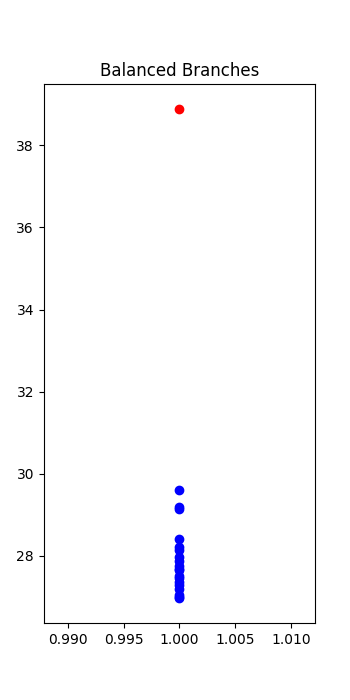
\includegraphics[width=.7\linewidth]{figures/branches0.png}
  \caption{With JIT}
  \label{fig:sub1}
\end{subfigure}%
\begin{subfigure}{.5\textwidth}
  \centering
  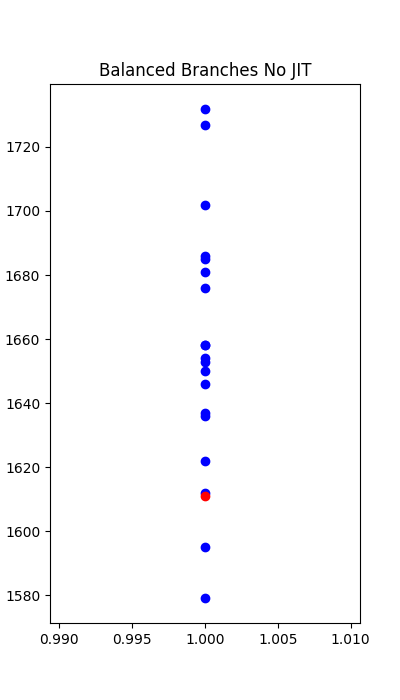
\includegraphics[width=.7\linewidth]{figures/nJITbranch1.png}
  \caption{Without JIT}
  \label{fig:sub2}
\end{subfigure}
\caption{Comparison of side-channel vulnerability for the balanced path \texttt{PassswordChecker} with and without JIT enabled. In each figure, the dots are each the time taken for a sample parameterized by the first character of the user guess. The red data point is the resulting time when the first character of the guess matches that of the secret.}
\label{fig:test}
\end{figure}

\begin{figure}
\centering
\begin{subfigure}{.5\textwidth}
  \centering
  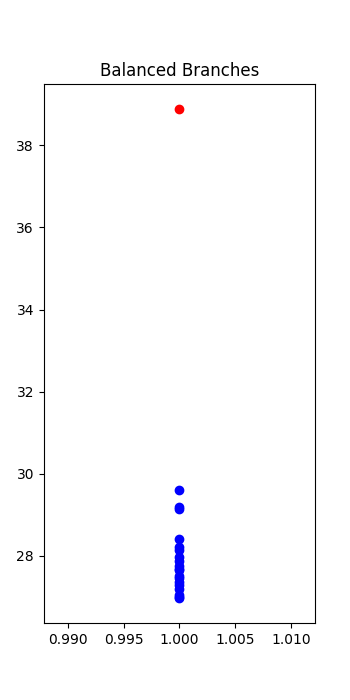
\includegraphics[width=.7\linewidth]{figures/branches0.png}
  \caption{Original input distribution}
  \label{fig:sub1}
\end{subfigure}%
\begin{subfigure}{.5\textwidth}
  \centering
  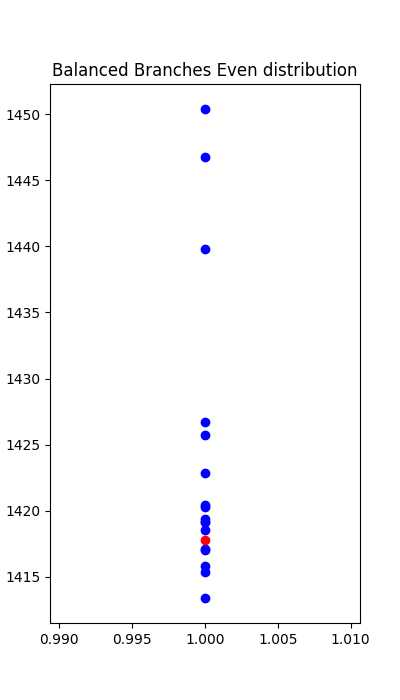
\includegraphics[width=.7\linewidth]{figures/distribution_branches2.png}
  \caption{Modified input distribution}
  \label{fig:sub2}
\end{subfigure}
\caption{Comparison of side-channel vulnerability for the balanced path \texttt{PassswordChecker} with a modified input distribution versus the original. In each figure, the dots are each the time taken for a sample parameterized by the first character of the user guess. The red data point is the resulting time when the first character of the guess matches that of the secret.}
\label{fig:test}
\end{figure}

\begin{figure}
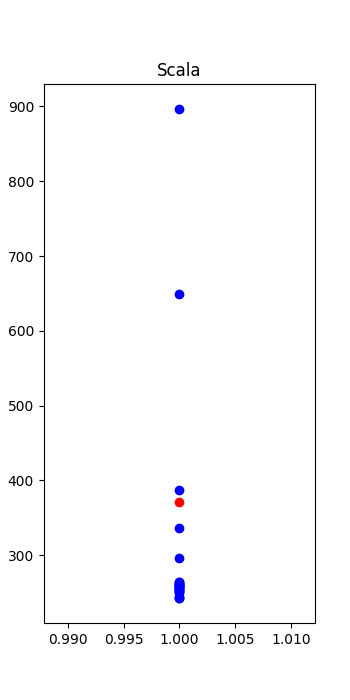
\includegraphics[scale=1]{figures/scala.png}
\caption{Results of the side-channel vulnerability for our scala implementation.}
\end{figure}

